Un \textbf{sistema a tempo discreto (TD) SLS o LTI} è un sistema che risulta essere contemporaneamente lineare e stazionario. In particolare, un sistema si dice \textbf{lineare} se ad una combinazione lineare degli ingressi corrisponde la combinazione lineare delle uscite (\textit{Principio di Sovrapposizione degli Effetti}):
\begin{equation}
    \alpha x_1 + \beta x_2 \overset{\tau}{\longrightarrow} \alpha y_1 + \beta y_2
\end{equation}
Invece, un sistema TD si dice \textbf{stazionario} (o tempo-invariante) se ritardando/anticipando l'ingresso di una quantità $n_0$ l'uscita viene ritardata/anticipata della stessa quantità:
\begin{equation}
    x[n-n_0] \overset{\tau}{\longrightarrow} y[n-n_0]
\end{equation}
Un sistema SLS-TD è caratterizzato dalla sua risposta impulsiva $h[n]$. Essa rappresenta l'uscita del sistema quando all'ingresso viene applicato un impulso discreto. 
\begin{center}
    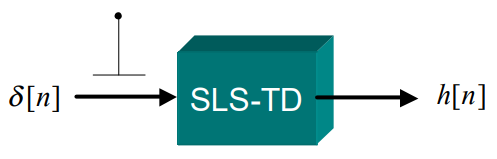
\includegraphics[width=0.5\textwidth]{introduction/rispostaimpulsiva.png}
\end{center}
Conoscendo la risposta impulsiva h[n] e applicando le proprietà di linearità e stazionarietà, è possibile calcolare l'uscita $y[n]$ corrispondente ad un qualunque ingresso $x[n]$:
\begin{equation}
    y[n] = \sum_{k=-\infty}^{+\infty} x[k] h[n-k] = x[n] \ast h[n]
\end{equation}
Pertanto, l'uscita si ottiene effettuando la convoluzione tra l'ingresso e la risposta impulsiva.
